\chapter{Week 6: Arduino met Pi Koppelen}

In deze laatste week van het Programmeren 2, gaan we ons eerst nog wat verder verdiepen in de wereld van object geörienteerd programmeren (OOP). Daarnaast stevenen we af op onze eindopdracht van dit vak (en eigenlijk ook van Programmeren 1).

\section{Overerven}\index{Overerven}
Met het vorige hoofdstuk heb je je eerste introductie gehad in de wereld van OOP. We hebben op een nieuwe abstracte manier naar problemen gekeken. Ook werd er toen verteld over de voordelen van OOP, zo kon je de code makkelijk onderhouden (je hoeft maar op $1$ plek de klasse-definitie/blauwdruk aan te passen, en overal waar je 'm gebruikt wordt deze verandering overgenomen). Maar ook werd er gesteld dat de gemaakte code eenvoudig uitbreidbaar is. Als we nu ons geheugen opfrissen door even te kijken naar de gemaakte \pyth{Cirkel}-klasse:

\inputpython{code/chapter08/cirkel.py}

We hadden een klasse \pyth{Cirkel} gemaakt die als eigenschap z'n straal had, en waarop we de functies \pyth{bereken_oppervlakte()} en \pyth{bereken_omtrek()} op kunnen uitvoeren. We kunnen nu deze klasse-definitie nu ook gebruiken om andere klasse te definiëren die gebasseerd zijn op deze cirkel. \newline 

Als we bijvoorbeeld een klasse willen maken voor een \pyth{Bol} en we gaan hiervoor beredeneren wat zijn eigenschappen en z'n functies zijn. Zul je zien dat deze veel zullen overeenkomen met die van de \pyth{Cirkel}. Qua eigenschappen kunnen we een bol definieren op basis van een straal en op basis van die straal kunnen we de omtrek, oppervlakte en inhoud van de bol berekenen. Grafisch weergegeven:
\begin{figure}[h!]
\centering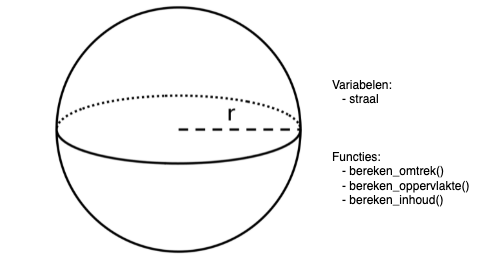
\includegraphics[scale=0.7]{Pictures/chapter08/bol.png}
\caption{Ons bol-object heeft een straal, en kan (op basis daarvan) de omtrek, oppervlakte en inhoud van zichzelf berekenen.}
\label{fig:bol} % Unique label used for referencing the figure in-text
%\addcontentsline{toc}{figure}{Figure \ref{fig:webserver}} % Uncomment to add the figure to the table of contents
\end{figure}

Zowel de klasse=variabele \pyth{r}, als $2$ van de $3$ functies\footnote{Wellicht heb je 'm al door: de oppervlakte van een bol berekenen je op een andere manier dan van een cirkel, hier komen we later op terug} komen overeen met die van \pyth{Cirkel}. Als we dus een klasse-definitie voor een \pyth{Bol} willen maken is het handiger om te baseren op een \pyth{Cirkel} dan helemaal opnieuw te beginnen, dat scheelt werk! Onze klasse-definitie van een \pyth{Bol} ziet er dan zo uit:

\inputpython{code/chapter08/bol.py}

Valt het je op hoe kort dit bestand is? Op regel $5$ gebeurt alle 'magie', hier wordt namelijk gesteld dat we een nieuwe klasse genaamd \pyth{Bol} willen maken, maar dat we deze willen baseren op \pyth{Cirkel}. \textit{Python} regelt nu onderwater dat de bol-klasse een klasse-variabele \pyth{r} voor de straal krijgt, en ook kan hij gebruik maken van de functies (waaronder de constructor) die in \pyth{Cirkel} zitten. \newline

Het enige wat wij zelf nog moeten doen is de nieuwe functie uitschrijven die de inhoudt van de bol berekend op basis van z'n straal, met de volgende formule: $V_{bol} = \frac{4}{3} \pi r^3$. \newline

\begin{remark}
Een klasse basseren op een andere klasse noemen we ook wel een \textit{subklasse} maken. \pyth{Bol} is in dit geval een subklasse van \pyth{Cirkel}. Andersom is \pyth{Cirkel} de \textit{superklasse} van \pyth{Bol}.
\end{remark}

Deze klasse-definitie kunnen we daarna gebruiken in andere programma's op de bekende manier:
\begin{python}
from bol import Bol

mijn_bol = Bol(10)  # Maak een bol aan met een straal van 10.

omt = mijn_bol.bereken_omtrek()
opp = mijn_bol.bereken_oppervlakte()
inh = mijn_bol.bereken_inhoud()

print(f"Omtrek: {omt:.2f}")
print(f"Oppervlakte: {opp:.2f}")
print(f"Inhoud: {inh:.2f}")
\end{python}

Wat het onderstaande als uitvoer geeft:
\begin{python}
Omtrek: 62.83
Oppervlakte: 314.16
Inhoud: 4188.79
\end{python}

In onze \pyth{Bol} zit echter nog wel een bug, de oppervlakte van een bol, bereken je op een andere manier dan van een cirkel. Voor een cirkel geldt: $O_{cirkel} = \pi r^2$, voor een bol: $O_{bol} = 4\pi r^2$. \newline

Gelukkig kunnen we in een subklasse functies van de superklasse makkelijk overschrijven:
\inputpython{code/chapter08/bol2.py}

Als we nu onze \pyth{Bol} gebruiken, zoals boven aan deze pagina, komen er wel de juiste waardes uit:
\begin{python}
Omtrek: 62.83
Oppervlakte: 1256.64
Inhoud: 4188.79
\end{python}

% \section{Protocollen}\index{Protocollen}
% \subsection{UART}\index{UART}
% \subsection{HTTP}\index{HTTP}
% \subsection{MQTT?}\index{MQTT?}

% \begin{figure}[h!]
% \centering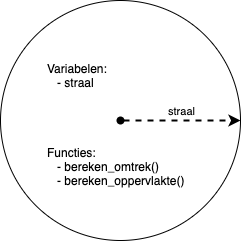
\includegraphics[scale=0.75]{Pictures/chapter07/cirkel.png}
% \caption{Ons cirkel-object heeft een straal, en kan (op basis daarvan) de omtrek en oppervlakte van zichzelf berekenen.}
% \label{fig:cirkel} % Unique label used for referencing the figure in-text
% %\addcontentsline{toc}{figure}{Figure \ref{fig:webserver}} % Uncomment to add the figure to the table of contents
% \end{figure}
%


% \newpage

% \section{Opdrachten}\index{Opdrachten}
% \begin{exercise}
% $\\$
% \end{exercise}

% \begin{exercise}
% $\\$
% \end{exercise}

% \begin{exercise}
% $\\$
% \end{exercise}

% \begin{exercise}
% $\\$
% \end{exercise}

% \begin{exercise}
% $\\$
% \end{exercise}

% \begin{exercise}
% $\\$
% \end{exercise}

% \begin{exercise}
% $\\$
% \end{exercise}

% \begin{exercise}
% $\\$
% \end{exercise}

